\section{DEPFET Pixel Sensors}
Contact person: Marcel Vos (email: vos@ific.uv.es)
\label{sec:DEPFET}
\subsection{The DEPFET Collaboration}
\href{http://www.hll.mpg.de/twiki/bin/view/DEPFET/CollaborationList}{The DEPFET collaboration} consists of nearly 100 members from 13 institutes. It currently takes responsibility for the following work packages:
\begin{description}
\item[Mechanics] {The DEPFET ladder integrates the support structure with the sensor wafer using state-of-the-art silicon processing technology. Read-out electronics and signal routing are integrated on the silicon wafer. The resulting all-silicon ladder is fully self-supporting. The mechanical properties of thin ladders in a realistic environment are studied in detail using detailed models (mock-ups) for Belle II and the ILC .}
\item[Cooling] {The DEPFET cooling concept for Belle II relies on two-phase \ce{CO2} cooling for the end-of-ladder. The sensor is cooled moreover with a forced flow of cold gas. The \ce{CO2} cooling plant is developed by KEK, while the design for the cooling block/support structure is performed within the collaboration. The impact of the linear collider cooling strategy - based on reducing the power dissipated using a pulsed power supply to the detector and cooling through a forced air flow - is studied. A novel cooling strategy for future applications based on mico-channels in the sensors is being evaluated in the collaboration. Solutions for monitoring of environmental parameters are being developed.}
\item[Ancillary ASICs] {The operation of a DEPFET detector requires ancillary electronics in the form of a read-out ASIC (the Drain Current Digitizer), a steering ASIC (SWITCHER) and on-detector ASICs for digital data processing (DHP). These ASICs are developed within the collaboration.}
\item[Data Acquisition and Trigger] {The development of off-detector electronics to process the data from the Belle II vertex detector.}
\item[Characterization of prototypes, laboratory and beam tests] {This work package has contributions from nearly all institutes involved in the DEPFET collaboration.}
\end{description}

Currently, the construction of the Belle II vertex detector~\cite{Abe:2010gxa} is the main focus of the collaboration. The requirements of the Belle II vertex detector are similar to those of the ILC, and more stringent in some aspects. The Belle II construction project therefore has considerable synergy with developments for a future linear collider. The LC-specific effort is focused on the development of small-pixel devices and the design of a forward vertex detector. We envisage that after the installation of the Belle II detector (2016) the balance between both projects is restored.

\begin{figure}
    \centering
    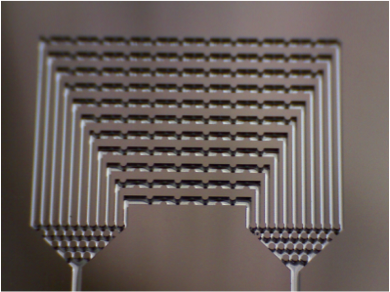
\includegraphics[width=.3\linewidth]{VertexDetector/DEPFET/microChannel}
    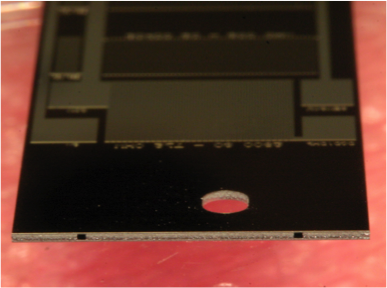
\includegraphics[width=.3\linewidth]{VertexDetector/DEPFET/microChannelSamples}
    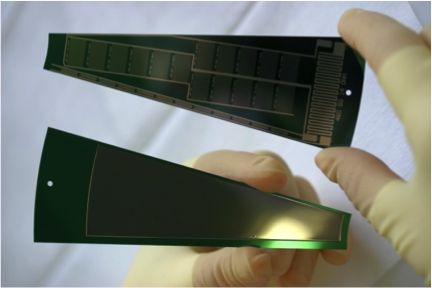
\includegraphics[width=.3\linewidth]{VertexDetector/DEPFET/FTD_Mockup}
    \caption{left: Microchannel cooling. center: Samples with cooling circuits. right: FTD mockup}
    \label{fig:VertexDetector:DEPFET}
\end{figure}

\subsection{Introduction}
The DEPFET technology implements amplification within the active pixel by integrating a p-MOS transistor in each pixel on the fully depleted high-resistivity silicon wafer. Additional n-implants near the transistor act as a trap for charge carriers created in the substrate (internal gate), so that they are collected beneath the transistor gate. The amplified signal is extracted from the pixel matrix by a numbers of ASICs~\cite{Kishishita:2014maa,Krueger2010337} mounted directly on the sensor: The SWITCHER, Drain Current Digitizer (DCD)~\cite{1748-0221-6-01-C01085,5446501} and Data Handling Processor (DHP)~\cite{1748-0221-7-01-C01069}.



The DEPFET in-pixel amplification allows for a comfortable signal-to-noise ratio with a very thin active detector. The reduced sensor thickness of $\SI{75}{\micro\meter}$ for Belle II, $\SI{50}{\micro\meter}$ for the Linear Collider, is the key to remain within the material budget of 0.15\% of a radiation length per layer. DEPFET prototypes with $20\times\SI{20}{\micro\meter\squared}$, small enough to meet the stringent spatial resolution specifications of the ILC, have successfully been operated in beam tests~\cite{Andricek:2011zza,Velthuis:2008zza}. The DEPFET matrix is read out in rolling shutter mode at a rate of 100 ns/row. For the column depths relevant for the ILC and Belle II a frame rate of several tens of $\si{\micro\meter}$ is achieved~\cite{6484214}. The expected performance of a DEPFET-based vertex detector meets the specifications drawn up by the ILD experiment. DEPFET is also considered as a back-up solution to the SiD concept, in case the single bunch crossing time stamping proves to be out of reach.



\begin{table}
\centering
\caption{Comparison of ILC and Belle II requirements of a vertex detector}
\label{tab:Vertex:DEPFET:ILCBelleComparison}
\begin{tabular}{ccc}
    & ILC & Belle II \\
    \hline
    occupancy & 0.13 hits/\si{\micro\meter\squared}/s & 0.4 hits/\si{\micro\meter\squared}/s \\
    radiation & $< \SI{100}{krad/yr}$ & $> \SI{1}{Mrad/yr}$  \\
    & $\SI{e11}{MeV n_{eq}/yr}$ & $2\times \SI{e12}{MeV n_{eq}/yr}$ \\
    duty cycle & 1/200 & 1 \\
    frame time & $25-\SI{100}{\micro s} $ & $\SI{20}{\micro s}$ \\
    momentum range & 100 keV - 500 GeV & $ < \sim\SI{1}{GeV}$ \\
    angular acceptance & 6\degree - 174\degree & 17\degree - 150\degree \\
    spatial resolution & excellent: $3-\SI{5}{\micro\meter}$ & moderate \\
    pixel size & $20\times \SI{20}{\micro\meter}$ & $50\times \SI{75}{\micro\meter}$ \\
    material budget & 0.15\% $X_0$/layer & 0.21\% $X_0$/layer \\
\end{tabular}
\end{table}

\subsection{Recent Milestones}
The concept of a DEPFET active pixel detector for vertex detection at collider experiments was initiated in the linear collider community (for TESLA).
The operation principle was extensively proven~\cite{Andricek:2011zza,Velthuis:2008zza} on small-scale prototypes. A recent reassessment of the DEPFET potential for a linear collider at the energy frontier is found in~\cite{6484214} and in the report~\cite{depfet:ecfaReport} for the ECFA detector R\&D review in 2014.
A large-scale, \SI{75}{\micro\meter} thin Belle II ladder with the ancillary ASICs integrated on the sensor was successfully submitted to a test in an electron beam at DESY in January 2014\cite{Marinas:2014iza}.


The first full-scale DHP prototype was implemented in IBM \SI{90}{nm} CMOS technology. As this technology was discontinued, more recent designs were submitted in the TSMC \SI{65}{nm} CMOS process. DHPT v.1.0 comprises temperature independent current references, 11 bias 8-bit DACs with current output, an integrated temperature measuring system and JTAG control. This design has been successfully tested during early 2014\cite{Kishishita:2014maa}.

\subsection{Engineering Challenges}
Vertex detector ladders with a thickness of several tens of microns and a spatial resolution of well below \SI{10}{\micro\meter} require very robust mechanical properties. The power generated by the sensors and ASICs must be removed with the smallest impact on the detector material.
Measurements on thin ladders under a realistic load, including pulsed powering according to the ILC beam structure, prove the excellent mechanical properties of the all-silicon ladder~\cite{thermomech}.

\subsection{Future Plans}
Currently, the construction of the Belle II vertex detector (to be installed by 2016 for the first physics run in 2017) implies a large effort of R\&D, including:
\begin{itemize}
\item Develop the die-attach technology in a controlled atmosphere required for the mounting of passive components on the DEPFET active pixel detector ladders. The first milestone is a fully integrated electrical prototype based on the EMCM.
\item First tests that will determine if all the ASICs on the ladder are fully functional
\item The integration of read-out and steering ASICs on the pixel sensor to be performed using a flip-chip technique and so-called bump-bonding, using microscopic solder balls.
\item The production of the Belle II vertex detector modules, a joint effort of the DEPFET collaboration
\item The test of the last version of the DHP chips
\end{itemize}
In the near future we hope to characterize the performance of a thin ILC-design prototypes with pixels of $20 \times \SI{20}{\micro\meter^2}$
\begin{itemize}
\item Perform an engineering design for a DEPFET all-silicon module with the required petal geometry
\item A detailed characterization of the response of the device
\item Design of the ancillary ASICs, taking full responsibility for future design cycles of the Front End read-out chip, the Drain Current Digitizer (DCD) that is relevant to the ILC and a Belle II upgrade. This chip converts the analog signal from the detector to digital and has a crucial impact on the detector performance.
\end{itemize}

In the longer term the DCD and DHP are envisaged to evolve into a single chip. Being large arrays of DEPFET pixels a promising technology for the vertex detector of the planned ILC, adaptation of the DCD and DHP chips must also be done.

 In the near future we hope to characterize the performance of ILC design prototypes with pixels of $20 \times \SI{20}{\micro\meter^2}$.
Important experience is furthermore gained with the thermal and mechanical properties of ultra-thin ladders. Measurents on thin ladders under a realistic load, including pulsed powering according to the ILC beam structure, prove the excellent mechanical properties of the all-silicon ladder. A complete mock-up for the innermost disks is under construction.
